% Beamer Presentation
% LaTeX Template
% Version 1.0 (10/11/12)
%
% This template has been downloaded from:
% http://www.LaTeXTemplates.com
%
% License:
% CC BY-NC-SA 3.0 (http://creativecommons.org/licenses/by-nc-sa/3.0/)
%
%%%%%%%%%%%%%%%%%%%%%%%%%%%%%%%%%%%%%%%%%

%----------------------------------------------------------------------------------------
%	PACKAGES AND THEMES
%----------------------------------------------------------------------------------------


	\documentclass[xcolor=dvipsnames]{beamer}

	\mode<presentation> {

	% The Beamer class comes with a number of default slide themes
	% which change the colors and layouts of slides. Below this is a list
	% of all the themes, uncomment each in turn to see what they look like.


	\usetheme{PaloAlto}

	% As well as themes, the Beamer class has a number of color themes
	% for any slide theme. Uncomment each of these in turn to see how it
	% changes the colors of your current slide theme.

	\usecolortheme{dove}


	%\setbeamertemplate{footline} % To remove the footer line in all slides uncomment this line
	%\setbeamertemplate{footline}[page number] % To replace the footer line in all slides with a simple slide count uncomment this line

	%\setbeamertemplate{navigation symbols}{} % To remove the navigation symbols from the bottom of all slides uncomment this line
	}

	\usepackage[spanish]{babel}
	\usepackage[utf8]{inputenc}

	\usepackage{graphicx} % Allows including images
	\usepackage{booktabs} % Allows the use of \toprule, \midrule and \bottomrule in tables
	\usepackage{multimedia}
	\usepackage{wrapfig}
	\usepackage{multicol}
	\usepackage{mathtools}
	\usepackage{subcaption}

	\usefonttheme{serif}

	%\setbeamersize{text margin left=0.5mm} 

	\setbeamercolor{frametitle}{bg=lightgray}
	\setbeamercolor{logo}{bg=gray}
	\setbeamercolor{section in sidebar}{fg=black} 
	\setbeamercolor{section in sidebar shaded}{fg=gray}
	\setbeamercolor{title}{fg=Black}
	\setbeamercolor{author in slidebar}{fg=black}

	\newcommand{\ibias}{I_{bias}}

%----------------------------------------------------------------------------------------
%	TITLE PAGE
%----------------------------------------------------------------------------------------

	\title[]{Simulación de peines de frecuencia óptica generados por láseres de semiconductor} % The short title appears at the bottom of every slide, the full title is onslide on the title page

	\author[Jaime Díez]{Jaime Díez González-Pardo } % Your name

	\institute[UC]{Universidad de Cantabria}

	\date{ \today} % Date, can be changed to a custom date

%----------------------------------------------------------------------------------------
%	Main Document
%----------------------------------------------------------------------------------------

	\begin{document}
	
		\begingroup
            \makeatletter
            \setlength{\hoffset}{-.5\beamer@sidebarwidth}
            \makeatother
            \begin{frame}[plain]
                    \vspace{1cm}
                    \begin{center}
                        {\fontsize{20pt}{24pt}\selectfont {Simulación de Peines de Frecuencia Óptica Generados por Láseres de Semiconductor}}
                    \end{center}
                    \vspace{1cm}

                \begin{columns}[onlytextwidth,T]
                    \column{\dimexpr\linewidth-35mm}%-5mm}
                        
                        \normalsize
                        	\textit{\tiny Autor:}

                            \insertauthor

                            \textit{\tiny Director:}

                            Ángel Valle

                    \column{35mm}
                        \includegraphics[width=25mm]{../download.png}

                \end{columns}
                
                \vspace{0.5cm}
                \begin{center}
                    \insertdate
                \end{center}
            \end{frame}
        \endgroup

		%\begin{frame}
		%	\titlepage % Print the title page as the first slides
		%\end{frame}

		\section{Láser de Semiconductor}
		%\graphicspath{{../Introduccion/Figures/}}

			% L\'aser de Semiconductor
			\begin{frame}
				\frametitle{\centerline{\textbf{L\'aser de Semiconductor}}}

				\vspace{-1.0cm}
				\begin{columns}
					\begin{column}{1.0\textwidth}
					\onslide<1->{
						\begin{figure}[H]
							\centering
							\includegraphics[width=1.0\linewidth, height=3.5cm]{Figuras/Bandas.png}
						\end{figure}}
					\end{column}
				\end{columns}
			
				%\vspace{-0.5cm}
				\begin{columns}
					\begin{column}{0.5\textwidth}
						\onslide<2->{L\'aser de Semiconductor:}
							\begin{itemize}
								\onslide<2->{\item Emisi\'on Lateral}
								\onslide<4->{\item Modo discreto (DML)}
							\end{itemize}
					\end{column}

					\begin{column}{0.5\textwidth}
						\onslide<3->{\begin{figure}[H]
									\centering
									\includegraphics[width=1.0\linewidth]{Figuras/Edge-Emitting.png}
								\end{figure}}
					\end{column}
				\end{columns}
			\end{frame}

			\subsection{OFC}

				% Peines de Frecuencia Óptica OFC
				\begin{frame}
					\frametitle{\centerline{\textbf{Peines de Frecuencia Óptica OFC}}}

					%\vspace{-0.9cm}
					\onslide<1->{
					\begin{figure}[H]
						\centering
						\includegraphics<1>[width=1.0\linewidth]{Figuras/OFC1.png}
						\includegraphics<2>[width=1.0\linewidth]{Figuras/OFC2.png}
						\includegraphics<3>[width=1.0\linewidth]{Figuras/OFC.png}
					\end{figure}
					}

					%\vspace{-0.5cm}
					\begin{columns}
						\begin{column}{0.4\linewidth}
							\onslide<1->{\begin{equation*}
									P(\omega) = \lim_{T\rightarrow\infty} |\mathcal{F}(x) (\omega)|^2 
							\end{equation*}								
							}
						\end{column}

						\begin{column}{0.2\linewidth}
							\onslide<2->{\begin{equation*}
								\delta\nu\delta t = \textrm{Cte}
							\end{equation*}
							}
						\end{column}

						\begin{column}{0.3\linewidth}
							\onslide<3->{\begin{equation*}
									\begin{matrix}
										x(t) = X_T(t) \ast S(t) \\ \\

										\chi(\nu) = \chi_T(\nu) \cdot S(\nu) 
									\end{matrix}
								\end{equation*}
							}
						\end{column}
					\end{columns}
					%\onslide<4->{Los efectos que se observan en los OFC son el resultado de la evolución de amplitud y fase óptica.}
				\end{frame}

				% M\'etodos de Generaci\'on de OFC
				\begin{frame}
					\frametitle{\centerline{\textbf{M\'etodos de Generaci\'on de OFC}}}

					\onslide<1->{Encendido por Ganacia (\textbf{Gain-Switching}):}
						\begin{itemize}
							\onslide<2->{\item Se alcanza rápidamente un alto valor para la ganancia del láser}
							\onslide<3->{\item Pulsos del láser de corta duración y grandes picos de potencia}
							%\onslide<4->{\item Se consigue que la inversi\'on de poblaci\'on, y por tanto la ganancia, alcance un valor muy por encima del valor umbral antes de que la densidad de fotones tenga tiempo de alcanzar un nivel suficiente para reducir la inversi\'on.}
						\end{itemize}

					\onslide<4->{\textbf{Inyecci\'on \'Optica}:}
						\begin{itemize}
							\onslide<5->{\item Inyectar fotones provenientes de un segundo láser}
							\onslide<6->{\item las caracter\'isticas de la fase del l\'aser inyectado pasan a estar determinadas por la inyecci\'on}
							\onslide<7->{\item Bloqueo por inyecci\'on}
						\end{itemize}
					\vspace{-1.1cm}
					\begin{columns}
						\begin{column}{0.4\textwidth}
							
						\end{column}

						\begin{column}{0.5\textwidth}
							\onslide<8->{\begin{figure}[H]
										\centering
										\includegraphics[width=1.0\linewidth]{Figuras/IL.png}
									\end{figure}}
						\end{column}
					\end{columns}
				\end{frame}

			\subsection{Ec. de Balance}

				% Ecuaciones de Balance
				\begin{frame}
					\frametitle{\centerline{\textbf{Ecuaciones de Balance}}}

					\onslide<1->{Densidad de Portadores:}
					\onslide<1->{\begin{equation*}
							\frac{\mathrm{d} N}{\mathrm{d} t} = \frac{I(t)}{e V_{act}} - R(N) - \frac{v_g \textrm{g}(N)S(t)}{1 + \epsilon S(t)} 
							\label{eq:RtEq-N}
						\end{equation*}}

					\onslide<2->{Densidad de Fotones:}
					\onslide<2->{\begin{equation*}
							\begin{matrix}
								\frac{\mathrm{d} S}{\mathrm{d} t} = & \left[ \frac{\Gamma v_g \textrm{g}(N)}{1 + \epsilon S(t)} - \frac{1}{\tau_p} \right] S(t) + \beta \Gamma BN^2 (t) \\ \\
								& + \sqrt{2 \beta \Gamma B N^2(t)S(t)} F_S(t) + Y_S(t)
							\end{matrix}
							\label{eq:RtEq-S}
						\end{equation*}}

					\onslide<3->{Fase \'Optica:}
					\onslide<3->{\begin{equation*}
							\begin{matrix}
							\frac{\mathrm{d} \Phi}{\mathrm{d} t} = & \frac{\alpha}{2}\left[ \Gamma
					        v_g \textrm{g}(N) - \frac{1}{\tau_p} \right] + 2\pi\Delta\nu(I) \\ \\
					        & + \sqrt{\frac{\beta \Gamma B N^2(t)}{2 S(t)}} F_{\Phi} (t) + Y_{\Phi}(t)
					        \end{matrix}
							\label{eq:RtEq-Ph}
						\end{equation*}
					}
				\end{frame}

			\subsection{Resoluci\'on estoc\'astica}

				% Resoluci\'on de EDS
				\begin{frame}
					\frametitle{\centerline{\textbf{Resoluci\'on de EDS}}}

					\begin{itemize}

						\onslide<1->{\item Las EDS vienen definidas por la ecuaci\'on de Langevin}

						\onslide<2->{\begin{equation*}
								\frac{\mathrm{d} x}{\mathrm{d} t} = a(x, t) + b(x, t) F(t)
							\end{equation*}}

						%\vspace{0.5cm}
						\onslide<3->{\begin{equation*}
											x(t+\Delta t) = x(t) + a(x, t)\Delta t + \eta(t)\sqrt{\Delta t}
									\end{equation*}
						}

						\onslide<4->{\item $\eta(t)$ es de tipo gaussiano con $\eta = \sqrt{V[\eta]} Z + E[\eta] = bZ$.}

						\onslide<5->{\begin{equation*}
								x_{i+1} = x_i + a(x_i, t_i)\Delta t + b(x_i, t_i) Z_i\sqrt{\Delta t}
							\end{equation*}}

					\end{itemize}
				\end{frame}

			\subsection{Dinamica No Lineal}

				% Din\'amica no lineal
				\begin{frame}
					\frametitle{\centerline{\textbf{Din\'amica no lineal}}}

					\begin{itemize}
						\onslide<1->{\item Comportamiento aleatorio y err\'atico, \textbf{Caos Determinista}}
						\onslide<2->{\item Se caracterian por la \textbf{\textit{divergencia de trayectorias cercanas}}}

						\onslide<3->{\item En los sitemas disipativos las trayectorias tienden al atractor}

						\onslide<4->{
							\begin{figure}[H]
								\centering
								\includegraphics<4>[width=0.8\linewidth]{Figuras/DnNoLi1.png}
								\includegraphics<5->[width=0.8\linewidth]{Figuras/DnNoLi.png}
							\end{figure}}

						\vspace{-0.7cm}
						\onslide<6->{\item Una bifurcaci\'on es el cambio en la soluci\'on debido al cambio en los par\'ametros}

					\end{itemize}
				\end{frame}

		\section{Láser en Solitario}
			\graphicspath{{../../Graphics/Cpt1-Charactz/}}

			% Espectros de Emisi\'on en CW
			\begin{frame}
				\frametitle{\centerline{\textbf{Espectros de Emisi\'on en CW}}}

				\begin{columns}
						\begin{column}{0.5\linewidth}
							\onslide<1->{\begin{figure}[H]
							\centering
							\includegraphics[width=1.0\linewidth]{Espectros.png}	
						\end{figure}							
							}
						\end{column}

						\begin{column}{0.5\linewidth}
							\onslide<2->{\begin{figure}[H]
							\centering
							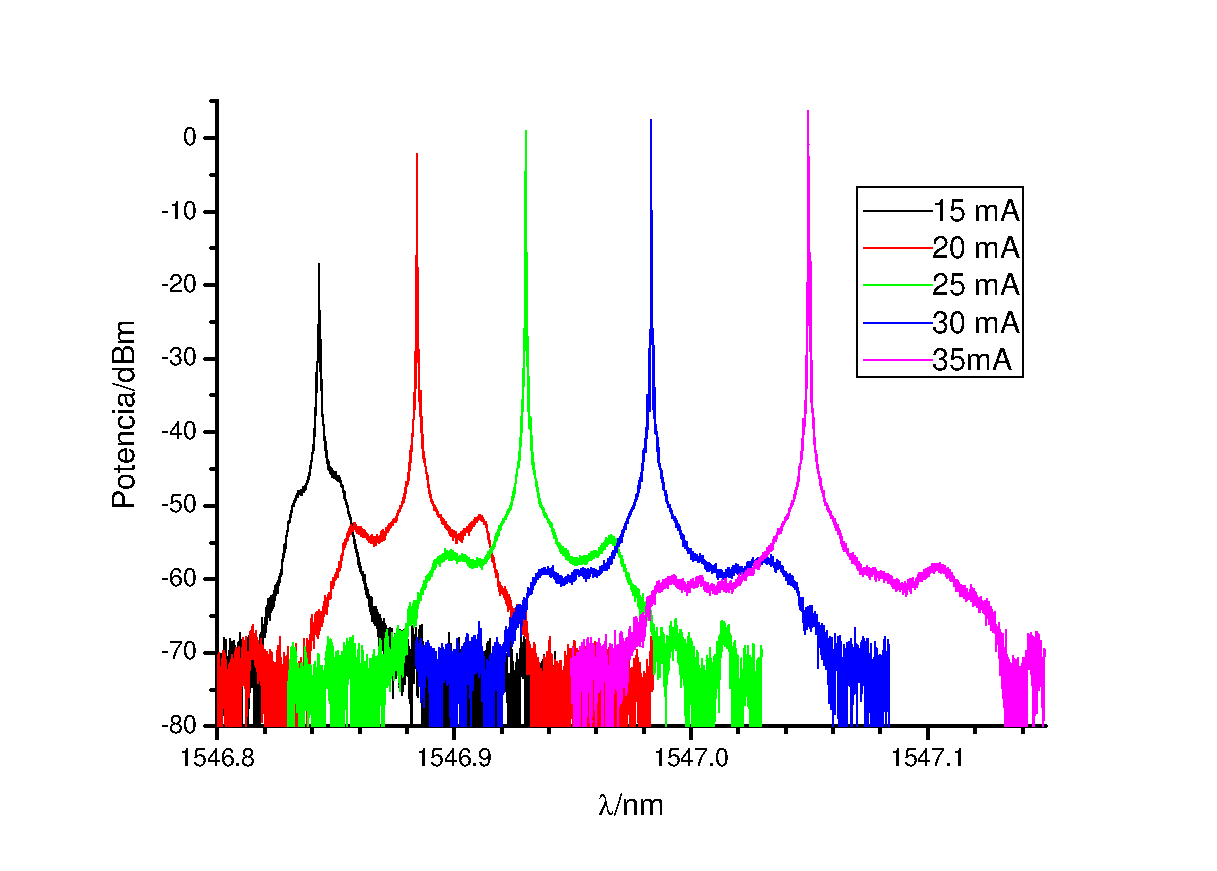
\includegraphics[width=0.9\linewidth]{../Chaves/OFC-GS/espectros_continua.png}
						\end{figure}
							}
						\end{column}
					\end{columns}				

				\begin{columns}
					\begin{column}{0.2\linewidth}
						\onslide<3->{\begin{equation*}
							\lambda_0 = \frac{2nL}{q}
							\label{eq:Cond}
						\end{equation*}
						}
					\end{column}

					\begin{column}{0.8\linewidth}
						\onslide<4->{
							\begin{table}[H]
								\centering
								\begin{tabular}{c c c}
									\hline
									$\ibias$ [mA] & $\lambda_{sim}$ [nm] & $\lambda_{exp}$ [nm] \\\hline 
									15 & 1546.86 & 1546.84 \\
									20 & 1546.90 & 1546.88 \\
									25 & 1546.94 & 1546.93 \\
									30 & 1546.99 & 1546.98 \\
									35 & 1547.05 & 1547.05 \\\hline
								\end{tabular}
							\end{table}
						}
					\end{column}
				\end{columns}
			\end{frame}

				
			\subsection{Encendido por Ganancia}

				% G-S a Altas Frecuencias $f_R = 5.0$ GHz
				\begin{frame}
					\frametitle{\centerline{\textbf{G-S a Altas Frecuencias $f_R = 5.0$ GHz}}}

					\onslide<1->{\begin{figure}[H]
							\centering
							\includegraphics[width=1.0\linewidth]{Figuras/RtEq.png}
						\end{figure}}
				\end{frame}

				% OFC en L\'aser Encendido por Ganancia
				\begin{frame}
					\frametitle{\centerline{\textbf{G-S a Altas Frecuencias $f_R = 5.0$ GHz}}}

					\onslide<1->{\begin{figure}[H]
							\centering
							\includegraphics[width=1.0\linewidth]{PSD.png}
						\end{figure}}
					
					\onslide<2->{Se observa la creaci\'on y destrucci\'on de los peines a medida que se aumenta la amplitud}
				\end{frame}

				%G-S a Bajas Frecuencias $f_R = 500$ MHZ
				\begin{frame}
					\frametitle{\centerline{\textbf{G-S a Bajas Frecuencias $f_R = 500$ MHz}}}

					\begin{columns}
						\begin{column}{0.5\linewidth}
							\onslide<1->{
								\begin{figure}[t]
									\centering
									\includegraphics[width=1.0\linewidth]{Figuras/LowFreq/Power(0,4-500m).png}
								\end{figure}
							}
						\end{column}
						\begin{column}{0.5\linewidth}
							\onslide<3->{
								\begin{figure}[t]
									\centering
									\includegraphics[width=1.0\linewidth]{Figuras/LowFreq/Power(1,2-500m).png}
								\end{figure}
							}
						\end{column}
					\end{columns}

					\begin{columns}
						\begin{column}{0.5\linewidth}
							\onslide<2->{
								\begin{figure}[t]
									\centering
									\includegraphics[width=1.0\linewidth]{Figuras/LowFreq/PSD(0,4-500m).png}
								\end{figure}
							}
						\end{column}
						\begin{column}{0.5\linewidth}
							\onslide<4->{
								\begin{figure}[t]
									\centering
									\includegraphics[width=1.0\linewidth]{Figuras/LowFreq/PSD(1,2-500m).png}
								\end{figure}
							}
						\end{column}
					\end{columns}
				\end{frame}

		\section{Inyecci\'on de Luz}

			% Inyecci\'on \'Optica
			\begin{frame}
				\frametitle{\centerline{\textbf{Inyecci\'on \'Optica}}}

				\vspace{-0.7cm}
				\onslide<1->{
					\begin{figure}[H]
						\hspace*{-1cm}
						%\centering
						\includegraphics<1>[width=1.1\linewidth]{Figuras/MapAnimation/Cpt4-PSD1.png}
						\hspace*{-0.1cm}
						\includegraphics<2>[width=1.1\linewidth]{Figuras/MapAnimation/Cpt4-PSD2.png}
						\hspace*{-0.1cm}
						\includegraphics<3>[width=1.1\linewidth]{Figuras/MapAnimation/Cpt4-PSD3.png}
						\hspace*{-0.1cm}
						\includegraphics<4>[width=1.1\linewidth]{Figuras/MapAnimation/Cpt4-PSD4.png}
						\hspace*{-0.1cm}
						\includegraphics<5>[width=1.1\linewidth]{Figuras/MapAnimation/Cpt4-PSD5.png}
					\end{figure}
				}
			\end{frame}

			%Bloqueo por Inyecci\'on y OFC
			\begin{frame}
				\frametitle{\centerline{\textbf{Bloqueo por Inyecci\'on y OFC}}}

				\onslide<1->{
					\begin{figure}[H]
						\centering
						\includegraphics[width=1.0\linewidth]{Figuras/Cpt4-RtEq.png}
					\end{figure}
				}
			\end{frame}

		\section{G-S con IO}

			% Inyecci\'on \'Optica en G-S
			\begin{frame}
				\frametitle{\centerline{\textbf{Inyecci\'on \'Optica en G-S}}}

				\onslide<1->{
					\begin{figure}[H]
						\centering
						\includegraphics[width=1.0\linewidth]{Figuras/Cpt5-p1-p2.png}
					\end{figure}
				}

				\onslide<2->{Se obtiene la bifurcaci\'on de doblamiento de periodo}
			\end{frame}

			% Inyecci\'on \'Optica en G-S
			\begin{frame}
				\frametitle{\centerline{\textbf{Inyecci\'on \'Optica en G-S}}}

				\onslide<1->{
					\begin{figure}[H]
						\centering
						\includegraphics[width=1.0\linewidth]{Figuras/Cpt5-chaos.png}
					\end{figure}
				}
			\end{frame}

		\section{Conclusiones}

			% Conclusiones
			\begin{frame}
				\frametitle{\centerline{\textbf{Conclusiones}}}

				\begin{itemize}
					\onslide<1->{\item Se ha observado la creaci\'on y destrucci\'on de los OFC en funci\'on de la amplitud. As\'i como la mayor irregularidad para bajas frecuencias.}

					\onslide<2->{\item Se han determinado las diferentes regiones din\'amicas para distintos valores de la inyecci\'on.}

					\onslide<3->{\item Se han obtenido bifurcaciones de Hopf y de doblamiento de periodo}

					\onslide<4->{\item El programa desarrollado permite entender mejor los procesos f\'isicos involucrados en la generaci\'on de OFC.}
				\end{itemize}
			\end{frame}

	%----------------------------------------------------------------------------
	%     Appendix
	%----------------------------------------------------------------------------	

		%Ruido Estoc\'astico
		\begin{frame}
			\frametitle{\centerline{\textbf{Ruido Estoc\'astico}}}

			\onslide<1->{Los términos de Langevin $F_S$ y $F_{\Phi}$ tienen las siguientes relaciones de correlación:}

			\onslide<2->{\begin{equation*}
				\left \langle F_i(t)F_j(t') \right \rangle = 2\delta_{ij}\delta(t-t')
			\end{equation*}

			\begin{equation*}
				\left \langle F_i(t) \right \rangle = 0
			\end{equation*}}

			\onslide<3->{Representan ruido blanco adicional debidos a la emisión espontánea}
		\end{frame}

		%Modelo Computacional
		\begin{frame}
			\frametitle{\centerline{\textbf{Modelo Computacional}}}

			\begin{itemize}

				%\onslide<1->{\item Se computan al comienzo de la simulaci\'on los par\'ametros y t\'erminos independientes de $N(t)$ y $S(t)$}

				\onslide<1->{\item Se realiza la transformada r\'apida de Fourier FFT por lo que el tiempo de la ventana ha de cumplir:}

					\onslide<1->{\begin{equation*}
						\frac{t_{Total}}{\Delta N} = 2^n
					\end{equation*}}

				\onslide<2->{\item Las frecuencias de la FFT realizada para un paso de $\Delta N$ viene dado por el intervalo:}

				\onslide<2->{\begin{equation*}
					[-\frac{1}{2\Delta N}, \frac{1}{2\Delta N})
				\end{equation*}}

				\onslide<3->{\item Hay que sumar una cantidad para que el espectro quede centrado en la frecuencia de emisi\'on $\nu$.}

				\onslide<3->{\begin{equation*}
					\nu_{th} - \frac{C(I)}{2\pi}
				\end{equation*}}
			\end{itemize}
		\end{frame}

		%Transitorio
		\begin{frame}
			\frametitle{\centerline{\textbf{Transitorio}}}

			\onslide<1->{\begin{figure}[H]
					\centering
					\includegraphics[width=0.9\linewidth]{transitorio.png}
				\end{figure}
			}
		\end{frame}

		%Doblamiento de Periodo en IL
		\begin{frame}
			\frametitle{\centerline{\textbf{Doblamiento de Periodo en IL}}}

			\onslide<1->{
				\begin{figure}[H]
					\centering
					\includegraphics[width=1.0\linewidth]{Figuras/Cpt4-ciclos.png}
				\end{figure}
			}
		\end{frame}

		%Inyecci\'on \'Optica en G-S
		\begin{frame}
			\frametitle{\centerline{\textbf{Inyecci\'on \'Optica en G-S}}}

			\onslide<1->{
				\begin{figure}[H]
					\centering
					\includegraphics[width=1.0\linewidth]{Figuras/Cpt5-psdMap.png}
				\end{figure}
			}
		\end{frame}


	%----------------------------------------------------------------------------
	%     BIBLIOGRAPHY
	%----------------------------------------------------------------------------

		\bibliographystyle{unsrt}
		\bibliography{../biblio}

	\end{document} 